\chapter{Overview}
\label{ch:detectors-overview}

%\section{Introduction to LBNF and DUNE}
% Intro shared by all subsections

\section{An International Physics Program}

The global neutrino physics community is developing a multi-decade
physics program to measure unknown parameters of the Standard Model of
particle physics and search for new phenomena.  The program will be carried out as an international,
leading-edge, dual-site experiment for neutrino science and proton decay studies, which 
is known as the Deep Underground Neutrino Experiment (DUNE).
The detectors for this experiment will be designed, built, commissioned and operated by the international DUNE Collaboration. The facility required to support this experiment, the Long-Baseline Neutrino Facility (LBNF), is hosted by Fermilab and its design and construction is organized as a DOE/Fermilab project incorporating international partners. Together LBNF and DUNE will comprise the world's highest-intensity neutrino beam at Fermilab, in Batavia, IL, a high-precision near detector on the Fermilab site, a massive liquid argon time-projection chamber (LArTPC) far detector installed deep underground at the Sanford Underground Research Facility (SURF) \SI{1300}{\km} away in Lead, SD, and all of the conventional and technical facilities necessary to support the beamline and detector systems. 


The strategy for executing the experimental program presented in this Conceptual 
Design Report (CDR) has been developed to meet the requirements 
set out in the P5 report~\cite{p5report} and takes into account the recommendations of the European Strategy for Particle Physics~\cite{ESPP-2012}. It adopts a model where U.S. and international funding agencies 
share costs on the DUNE detectors, and CERN and other participants provide in-kind contributions 
to the supporting infrastructure of LBNF. LBNF and DUNE will be tightly coordinated as DUNE collaborators 
design the detectors and infrastructure that will carry out the scientific program.
  
The scope of LBNF is
\begin{itemize}
\item an intense neutrino beam aimed at the far site
\item conventional facilities at both the near and far sites
\item cryogenics infrastructure to support the DUNE
  liquid argon time-projection chamber (LArTPC) detectors at SURF
\end{itemize}

The DUNE detectors include
\begin{itemize}
\item a high-performance neutrino detector and beamline monitoring system
located a few hundred meters downstream of the neutrino source
\item a massive LArTPC neutrino detector located deep underground at the far site
\end{itemize}

With the facilities provided by LBNF and the detectors provided by
DUNE, the DUNE Collaboration proposes to mount a focused attack on the
puzzle of neutrinos with broad sensitivity to neutrino oscillation
parameters in a single experiment.  The focus of the scientific
program is the determination of the neutrino mass hierarchy and the
explicit demonstration of leptonic CP violation, if it exists, by
precisely measuring differences between the oscillations of muon-type
neutrinos and antineutrinos into electron-type neutrinos
and antineutrinos, respectively. Siting the far detector deep underground will
provide exciting additional research opportunities in nucleon decay,
studies utilizing atmospheric neutrinos, and neutrino astrophysics,
including measurements of neutrinos from a core-collapse supernova
should such an event occur in our galaxy during the experiment's
lifetime.

%%%%%%%%%%%%%%%%%%%%%%%%%%%%%%%%%%%%%%%%%%%%%%%%%%%%%%%%%%%%%%%
\section{The LBNF/DUNE Conceptual Design Report Volumes}

%%%%%%%%%%%%%%%%%%%%%%%%%%%%%%%%%%%
\subsection{A Roadmap of the CDR}

The LBNF/DUNE CDR describes the proposed physics program and 
technical designs at the conceptual design stage.  At this stage, the design is
still undergoing development and the CDR therefore presents a \textit{reference design} 
for each element as well as \textit{alternative designs} that are under consideration.

The CDR is composed of four volumes and is supplemented by several annexes that 
provide details on the physics program and technical designs. The volumes are as follows

\begin{itemize}
\item \volintro{} provides an executive summary of and strategy for the experimental 
program and of the CDR as a whole.
\item \volphys{} outlines the scientific objectives and describes the physics studies that 
the DUNE Collaboration will undertake to address them.
\item \vollbnf{} describes the LBNF Project, which includes design and construction of the 
beamline at Fermilab, the conventional facilities at both Fermilab and SURF, and the cryostat
 and cryogenics infrastructure required for the DUNE far detector.
\item \voldune{} describes the DUNE Project, which includes the design, construction and 
commissioning of the near and far detectors. 
\end{itemize}

More detailed information for each of these volumes is provided in a set of annexes listed on the \href{https://web.fnal.gov/project/LBNF/ReviewsAndAssessments/LBNF-DUNE%20CD-1-Refresh%20Directors%20Review/SitePages/Home.aspx}{review website}. 

%%%%%%%%%%%%%%%%%%%%%%%%%%%%%%%%%%%
%\subsection{About this Volume}  <----- follows in overview chapter file of indiv volume




\section{About this Volume}

The first part of \voldune of the CDR describes the strategies for
implementing the near and far detectors
(Chapter~\ref{ch:detectors-strategy}) and outlines the DUNE management
structure (Chapter~\ref{ch:detectors-pm}). The next part describes the
technical designs: the reference and alternative designs for the far
detector and the synergies between them
(Chapters~\ref{ch:detectors-fd-ref},~\ref{ch:detectors-fd-alt}
and~\ref{ch:detectors-synergy}), and the near detector design
(Chapter~\ref{ch:detectors-nd-ref}).  Following this,
Chapter~\ref{ch:detectors-sc} describes the designs for the computing
infrastructure and physics software, which are not part of the DUNE Project, and
Chapter~\ref{ch:detectors-proto} provides an overview of the
prototyping efforts that are ongoing or
planned. Chapter~\ref{ch:detectors-summary} summarizes and concludes
the volume.
 

\section{Introduction to the DUNE Detectors}
\label{sec:intro-dune-det}

\subsection{Far detector}
\label{sec:intro-dune-far-det}

The proposed Far Detector (FD) will be located deep underground at the
SURF 4850L with a fiducial mass of 40-kt. It consists of four
identical cryostats instrumented with Liquid Argon Time Projection
Chambers (LArTPC) (See Figure~\ref{fig:FarDet-overview-SPDP}). The
LArTPC provides excellent tracking and calorimetry performance. It is
ideal for massive neutrino detectors which require high signal
efficiency and effective background discrimination, excellent
capability to identify and measure precisely neutrino events over a
wide range of energies, and excellent reconstruction of the kinematic
properties with a high resolution. The full imaging of events will
allow study of neutrino interactions and other rare events with
unprecedented detail. The huge mass will enable large data sets for
precision studies and the search for CP violation.

The LArTPC concept pioneered in the context of the ICARUS project, is
a mature technology with several decades of worldwide R\&D.
Nonetheless, the size of a single 10-kt DUNE module represents an
extrapolation by approximately one order of magnitude compared to the
largest operated detector, the ICARUS~T600. To address this challenge
DUNE is developing two far detector options, the reference and
alternate designs, and is engaged in a comprehensive prototyping
effort. At this stage, the development of two FD options is a strength
and an added-value made possible by the merging of the worldwide
neutrino community into DUNE.

\begin{cdrfigure}[3D models of the DUNE far detector designs]{FarDet-overview-SPDP}
{3D models of two 10-kt detectors using the single-phase reference design (left) 
and the dual-phase alternate design (right) for the DUNE far detector to be 
located at 4850L.}
\centering
\begin{minipage}[b]{1.0\textwidth}
\begin{center}
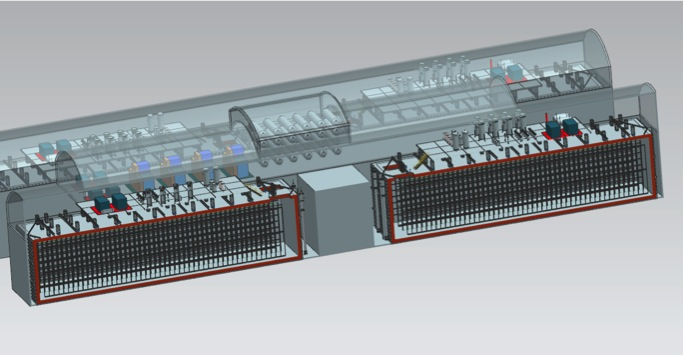
\includegraphics[width=.5\textwidth]{FarDet-3D-SP.jpg}
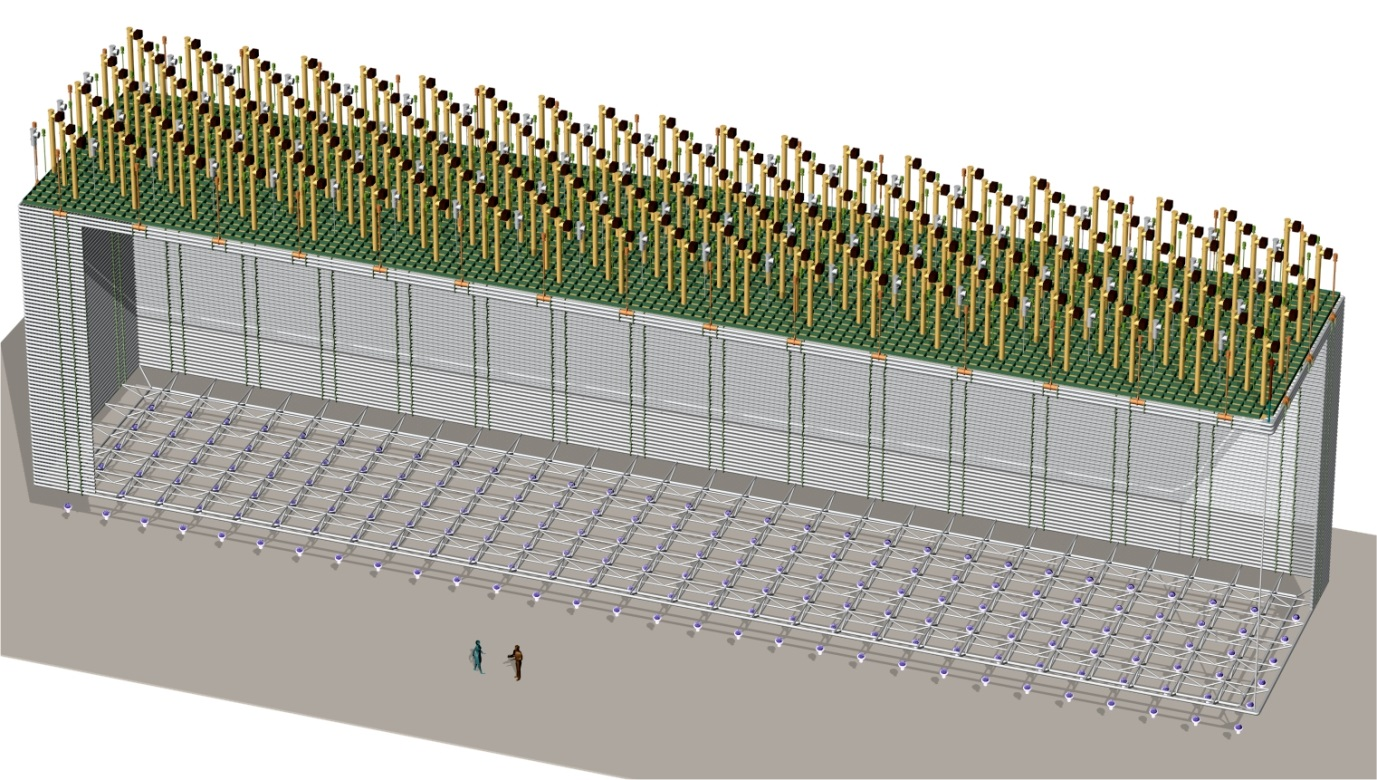
\includegraphics[width=0.46\textwidth]{DP_det2.jpg}
\end{center}
\end{minipage}
\end{cdrfigure}

Interactions in liquid argon produce ionization charge and
scintillation light.  The charge drifts in a constant electric field
away from the cathode plane towards the segmented anode plane.  The
prompt scintillation light is observed by photodetectors that provide
the absolute time of the event.  The reference design, described in
Chapter~\ref{ch:detectors-fd-ref}, adopts a single-phase readout,
where the readout anode is composed wire planes in the liquid argon
volume.  The alternate design, discussed in
Chapter~\ref{ch:detectors-fd-alt}, considers the dual-phase approach,
where ionization charge is extracted, amplified and detected in
gaseous argon above the liquid surface.  The dual phase design will
allow a finer readout pitch (3-mm), lower detection-energy threshold,
and better pattern reconstruction of the events.  The reference and
alternate design adopt complementary designs to collect the
scintillation light.

A comprehensive prototyping strategy for both designs is being actively
pursued as described in Chapter~\ref{ch:detectors-proto}.  The
reference design, closer to the original ICARUS design, is currently
being validated in the 35-t prototype LAr detector at Fermilab.  The
novel alternate design approach has been proven on
several small scale prototypes and a 20-t dual-phase
prototype is being constructed at CERN (WA105 3x1x1) to be
operated in 2016.  The ultimate validation of the engineered solutions
for both designs of the FD is foreseen at the CERN neutrino platform
around the year 2018, where full scale engineering prototypes will be
assembled and commissioned. After this milestone, a test beam data
campaign will be executed in the following years to collect large
sample of charge particle interactions to study the detector response
with high precision. A list of synergies
between the reference and alternative designs has been identified and
summarized in Chapter~\ref{ch:detectors-synergy}. Common solutions for
DAQ, electronics, HV feed-throughs, etc. will pursued and
implemented, independent of the details of the TPC design. These ongoing
efforts including those at the CERN Neutrino Platform will provide the ideal
environment to exploit these synergies and implement common solutions.

The deployment of the four 10-kt modules at SURF will take several
years with a vision guided by principles detailed in
Chapter~\ref{ch:detectors-strategy}. According to this strategy, the
Collaboration will adopt the lowest-risk design that satisfies the
physics and detector requirements in order to start the
installation of the first FD 10-kt module as early as possible.
The first 10-kt module will implement the reference design. %, subject to risks identified in the register.  
Installation of the second 10-kt module will commence
soon thereafter.  Hence, the second cryostat should be
instrumented as soon as possible.  There is recognition that
LArTPC technology will continue to evolve with (1) the large-scale
prototypes at the CERN Neutrino Platform and the experience from the
Fermilab SBN program, and (2) the experience gained during the
construction and commissioning of the first 10-kt module.  It is
assumed that all four detector modules will be similar but not
necessarily identical, allowing for evolution of the LArTPC
technology to be implemented in the FD detectors. There will be a
clear and transparent decision process for the design of the second
and subsequent modules, allowing for implementation of evolving LArTPC
technologies. The decision will be based on physics performance,
technical and schedule risks, costs, and funding opportunities.  A
flexible approach to the DUNE far detector design is the ideal
response to the diversity of the Collaboration and offers the
potential to attract additional interest and resources into the
Collaboration. A staged approach provides access to an early science
program while allowing for improvements and developments to be
implemented during the life of the experiment.

\subsection{Near detector}
\label{sec:intro-dune-near-det}

The spectrum and flavor composition of the neutrino beam will be
measured with high precision in order to reach the ultimate
sensitivity for the long-baseline neutrino oscillation studies.  The
separation between fluxes of neutrinos and antineutrinos requires a
magnetized neutrino detector to charge discriminate electrons and
muons produced in the neutrino charged current interactions.  This is
the primary role of the DUNE near detector system; however, exposure
to the intense neutrinos flux provides the opportunity to collect
unprecedentedly high neutrino interaction statistics for an extended
science program.  The near detector will therefore provide an
opportunity for a wealth of fundamental neutrino interaction
measurements, which are an important part of the secondary scientific
goals of the DUNE collaboration.  The reference design for the
neutrino near detector (NND) design is the NOMAD-inspired fine-grained
tracker (FGT) and is described in
Chapter~\ref{ch:detectors-nd-ref}. The NND subsystems include a
central straw-tube tracker and an electromagnetic calorimeter embedded
in a 0.4-T dipole field. The magnet yoke steel will be instrumented
with muon identifiers.

The near detector system will be complemented with a Beamline
Measurement System (BLM) located in the region of the beam absorber at
the downstream end of the decay region. BLM aims to measure the muon
flux from hadron decay.  The BLM is intended to monitor the beam
profile on a spill-by-spill basis and will operate for the life of
the experiment.
